\documentclass{article}
\usepackage{lmodern} % Fix the font size warnings
\usepackage{fancyhdr} % Required for custom headers
\usepackage{lastpage} % Required to determine the last page for the footer
\usepackage{extramarks} % Required for headers and footers
\usepackage{graphicx} % Required to insert images
\usepackage{mathabx} % Required for hash sign
\usepackage{xfrac} % Nice fractions

\usepackage{multicol}

% Margins
\topmargin=-0.5in
\evensidemargin=0in
\oddsidemargin=-0.5in
\textwidth=7.5in
\textheight=9.0in
\headsep=0.25in 

% paragraphs
\usepackage{parskip}

\pagestyle{fancy}

\rhead{Desserts and sweets}
\lhead{\textbf{Snickerdoodles}}
\chead{}
\title{Snickerdoodles}

\begin{document}

Like many of our recipes, this one started off in Cook's Illustrated Baking, but\dots it really
ended up being ours after several iterations. You see, Dad can't stop messing with recipes and will
keep tweaking them until they're \textit{just right}.

What makes this a better snickerdoodle is the addition of cinnamon and allspice to the
dry ingredients in addition to that in which the cookies are rolled.

\begin{figure}
    \centering
    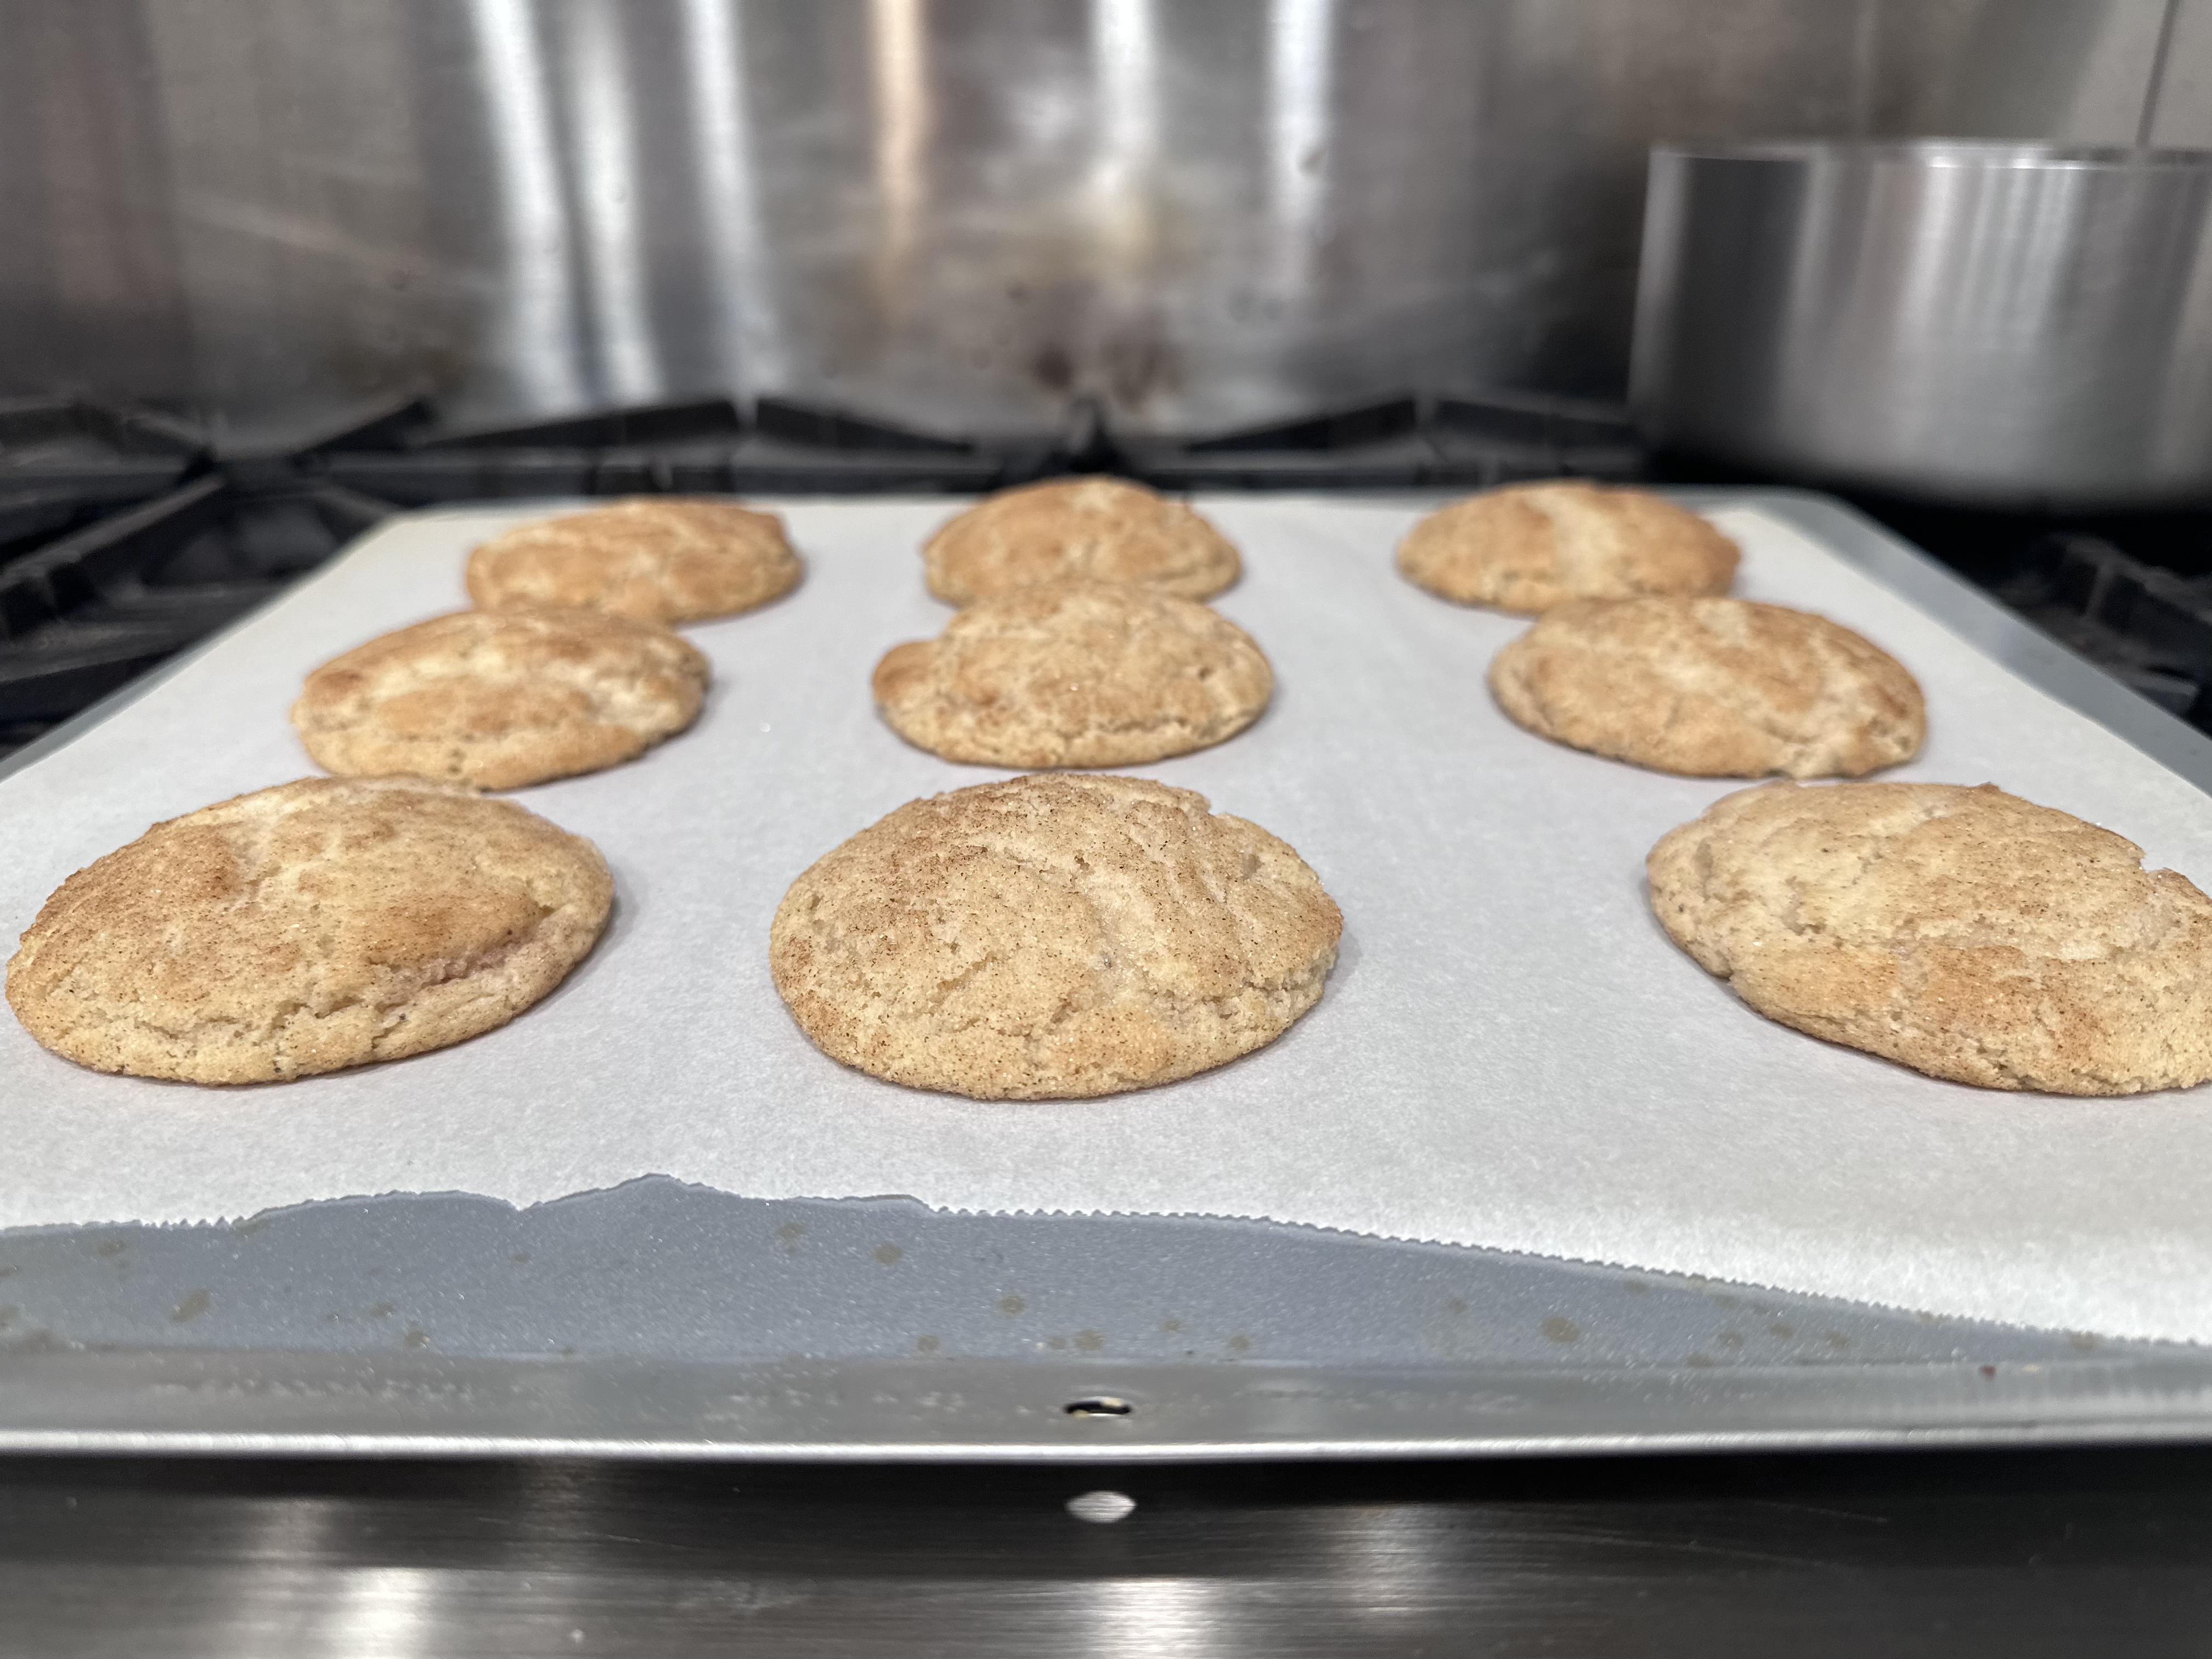
\includegraphics[scale=0.025]{snickerdoodles.png}
\end{figure}

\textbf{Ingredients}

\begin{multicols}{2}
    \begin{itemize}
        \item 2\sfrac{1}{2} cups all purpose flour
        \item 2 teapoons cream of tartar
        \item 1 teaspoon baking soda
        \item \sfrac{1}{2} teapoon salt
        \item 2 teaspoons cinnamon
        \item \sfrac{1}{4} teapoon allspice

        \item 1\sfrac{1}{2} sticks butter (12 tablespoons), at room temperature
        \item \sfrac{1}{4} vegetable shortening, at room temperature
        \item 1\sfrac{1}{2} cup granulated sugar, plus 3 tablespoons for rolling
        \item 2 large eggs, at room temperature
        \item 1 tablespoon cinnamon plus \sfrac{1}{3} cup granulated sugar for rolling
    \end{itemize}
\end{multicols}

\textbf{Directions}

\begin{enumerate}
    \item Preheat oven to 400 degrees.
    \item Whisk the flour, cream of tartar, baking soda, salt, allspice, and the 2 teapoons cinnamon
          in a small bowl.
    \item Mix the butter, shortening, and sugar together until just combined. DO NOT overmix. Run at
          medium speed, for about 1\sfrac{1}{2} minutes.
    \item Add the eggs and blend until just combined.
    \item Add the dry ingredients to the mixer and mix until dough is smooth.
    \item Using a small $\varhash 20$ scoop, drop the dough into the sugar and cinnamon mixture and
          evenly coat.
    \item Put the dough rounds on a jelly roll pan and chill at least one hour.
    \item Bake until the edges of the cookies are beginning to set and the centers are soft
          and puffy, about 9 minutes. Let the cookies cool on the baking sheets for 2 to 3
          minutes then move to a wire rack. The cookies might appear slightly under done. This
          is expected and ok.
\end{enumerate}

\medskip

% I suppose pictures could go here

\end{document}
